\documentclass[a4paper, 12pt]{article}%тип документа

%отступы
\usepackage[left=2cm,right=2cm,top=2cm,bottom=3cm,bindingoffset=0cm]{geometry}
\setlength{\parindent}{5ex}

%Русский язык
\usepackage[T2A]{fontenc} %кодировка
\usepackage[utf8]{inputenc} %кодировка исходного кода
\usepackage[english,russian]{babel} %локализация и переносы

%Вставка картинок
\usepackage{graphicx}
\graphicspath{{pictures/}}
\DeclareGraphicsExtensions{.pdf,.png,.jpg}

%Графики
\usepackage{pgfplots}
\pgfplotsset{compat=1.9}

%Математика
\usepackage{amsmath, amsfonts, amssymb, amsthm, mathtools}

%Таблицы
\usepackage{longtable} 
\usepackage{float}

%Римские цифры
\newcommand{\RomanNumeralCaps}[1]{\uppercase\expandafter{\romannumeral#1}}

\usepackage{multirow}


\begin{document}
	\begin{titlepage}
		\begin{center}
			\textsc{Федеральное государственное автономное образовательное учреждение высшего образования«Московский физико-технический институт (национальный исследовательский университет)»\\[5mm]
			}
			
			\vfill
			
			\textbf{Вопрос по выбору: \\[3mm]
			Дробовой шум.
				\\[50mm]
			}
			
		\end{center}
		
		\hfill
		\begin{minipage}{.5\textwidth}
			Выполнил студент:\\[2mm]
			Сериков Василий Романович\\[2mm]
			Группа: Б03-102\\[5mm]
			
		\end{minipage}
		\vfill
		\begin{center}
			Москва, 2022 г.
		\end{center}
		
	\end{titlepage}
	
	\newpage
	\textbf{Аннотация}\\
	
	
	\textbf{Цель работы: }\\
	Измерение заряда электрона по дробовому шуму.\\
	
	\textbf{В работе используется: }\\
	Стенд для измерения дробового шума, состоящий из шумового диода, блока питания, широкополосного усилителя, квадратичного детектора и кварцевого генератора синусоидальных колебаний.\\
	
	\textbf{Теоретические сведения: }\\
	
	Прохождение электрического тока через вакуумную
	лампу обусловлено с движением электронов, испускаемых накалённым
	катодом и движущихся к аноду под действием электрического поля. Прохождение электрического тока не является поэтому непрерывным процессом. Ток состоит из наложения кратковременных импульсов, возникающих при прохождении отдельных электронов. Эти импульсы случайным образом распределены во времени, вследствие чего электрический
	ток флуктуирует. При этом на средний (постоянный) ток накладывается
	флуктуационный шум, связанный с дискретностью заряда электронов —
	\textit{дробовой шум}. Анализ этого шума — один из немногих способов измерения абсолютного заряда электрона. Флуктуации анодного тока — при заданной его величине — пропорциональны заряду электрона, поэтому, исследуя их, можно измерить заряд электрона.
	
	Рассмотрим, как меняется во времени ток, проходящий во внешней
	цепи электронной лампы (диода) при движении через неё отдельного
	электрона. Пока из катода не вылетит электрон, тока в цепи лампы нет.
	Ток появляется, когда электрон покидает катод, и кончается, когда он
	приходит на анод. Распределение этого тока во времени носит сложный
	характер, зависящий от геометрии электродов, от распределения потенциалов в межэлектродном пространстве и от скорости электронов.
	В дальнейшем нас не будет интересовать форма токового импульса. Нам достаточно знать, что этот импульс является кратковременным
	($\sim 10^{-8}$ с) и что за время этого импульса $\int I dt = e$, где e — заряд электрона. Будем рассматривать режим насыщения диода, когда пространственный заряд в межэлектродном пространстве отсутствует и анодный	ток зависит только от количества электронов, испущенных катодом.
	Для обнаружения дробового шума в анодную цепь лампы включена нагрузка — параллельный колебательный контур (рис. 1).
	
	\begin{figure}[H]
		\center{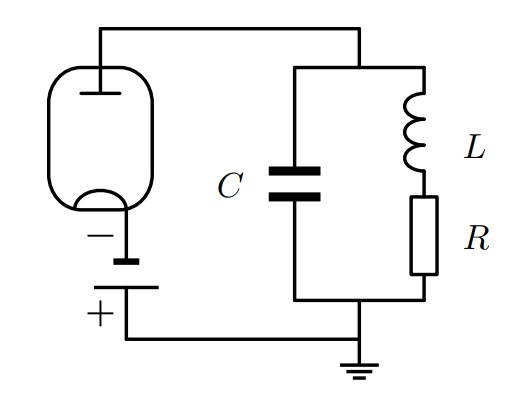
\includegraphics [scale=0.7]{LCR.png}}
		\caption{Схема включения LCR-контура.}
	\end{figure}
	
	Токовый
	импульс, связанный с прохождением электрона через диод, приводит к
	зарядке конденсатора C, который входит в состав LCR-контура. В контуре возникают электрические колебания. Следующие электроны — в
	зависимости от фазы колебаний контура — усиливают или ослабляют колебательный процесс. Постепенно в контуре возбуждаются колебания,
	амплитуда и фаза которых случайным образом меняются во времени.
	Кроме заряда, связанного с колебательным процессом, на конденсаторе
	есть, конечно, заряд, возникающий из-за наличия среднего тока. Этот заряд нас интересовать не будет. Среднее значение амплитуды колебаний
	контура может быть найдено из энергетических соображений. Установившееся значение амплитуды определяется тем, что средняя энергия,
	которую приносят электроны на конденсатор, равна энергии, которая
	рассеивается в колебательном контуре.
	Пусть при электрических колебаниях в контуре мгновенное значение
	напряжения на конденсаторе равно
	
	\begin{equation}
		U = U_0 \cos(\omega t) 
	\end{equation}
	До пролёта очередного электрона заряд на конденсаторе равен
	$q_1 = CU_0 \cos(\omega t)$, а после пролёта он принимает значение $q_2$:
	
	\begin{equation}
	q_2 = q_1 + e
	\end{equation}
	Приход электрона увеличивает энергию конденсатора на $\Delta W$:
	
	\begin{equation}
		\Delta W = \frac{2eCU_0\cos(\omega t) + e^2}{2C}
	\end{equation}
	Пусть в секунду через лампу проходят N электронов. Полное увеличение средней энергии конденсатора складывается из N слагаемых,
	определяемых формулой (3). При этом вклад от первого члена формулы обращается в нуль, так как электроны приходят на конденсатор в произвольные моменты времени, а среднее значение $\cos(\omega t)$ равно нулю.
	Средняя мощность, приносимая электронами на конденсатор, определяется поэтому только вторым слагаемым и равна $P$:
	 
	\begin{equation}
		P = N \frac{e^2}{2C} 
	\end{equation}
	
	Рассчитаем теперь потери в сопротивлении. Проходящий через него
	ток $IR$ складывается из постоянного тока $I_=$ и колебательного тока контура $I_{\sim}$. Выделяемая в сопротивлении мощность в среднем равна
	
	\begin{equation}
		\langle P_R \rangle = \langle I^2R \rangle = R \langle(I_= + I_{\sim})2 \rangle
	\end{equation}
	
	Зная, что среднее значение $\langle \sin(\omega t) \rangle = 0$, а
	$\langle \sin^2(\omega t) \rangle = 1/2$ и $I_{\sim} = dq/dt $ найдём
	
	\begin{equation}
		\langle P_R \rangle = RI^2_= + R\langle I^2_{\sim} \rangle = RI^2_= + \frac{1}{2} RC^2U_0^2\omega^2
	\end{equation}
	
	Приравняем мощность (4), возбуждаемую электронами в контуре, к
	мощности  $R\langle I^2_{\sim} \rangle$, теряемой в сопротивлении из-за наличия колебаний. Заметив, что $Ne = I_a$, а амплитудное значение напряжения на конденсаторе $U_0$ связано с эффективным значением $U_{\text{эфф}}$ обычным соотношением $U_{\text{эфф}} = U_0^2/2$, найдём для заряда электрона e следующую формулу:
	
	\begin{equation}
		e = \frac{2\omega^2RC^3U_{\text{эфф}}^2}{I_a}
	\end{equation}
	
	Можем записать выражение для e через добротность контура $Q = 1/\omega RC$
	
	\begin{equation}
		e = \frac{4\pi f C^2U_{\text{эфф}}^2}{QI_a}
	\end{equation}
	
	\textbf{Экспериментальная установка: }\\
	
	Блок-схема установки изображена на рис 2. В качестве шумового диода используется диод 2Д3Б, работающий в режиме насыщения. В его
	анодную цепь включён параллельный колебательный контур LC. Активное сопротивление катушки L играет роль резистора R. Конденсатор C непосредственно включён в цепь контура при нижнем положении
	переключателя $"U_k"$ (его кнопка не нажата). Измерение напряжения
	на контуре производится квадратичным детектором (отклик которого
	пропорционален квадрату напряжения). Перед измерениями сигнал, поступающий с контура, усиливается усилителем. Также используется генератор для калибровки квадратичного детектора и для измерения добротности контура.
	
	Выходное напряжение генератора $U_{\text{г}}$ целиком падает на активном сопротивлении контура R. Поэтому $U_{\text{г}}$ = RI, где I — ток в контуре. Найдём теперь напряжение $U_k$, подаваемое на усилитель и измеряемое квадратичным детектором:
	$$U_k = U_{\text{г}} - \frac{I}{\dot\imath \omega C} \approx \frac{\dot\imath U_{\text{г}}}{\omega RC}$$
	
	Тогда добротность контура:
	$$ Q =  \frac{U_k}{U_{\text{г}}}$$
	
	\begin{figure}[H]
		\center{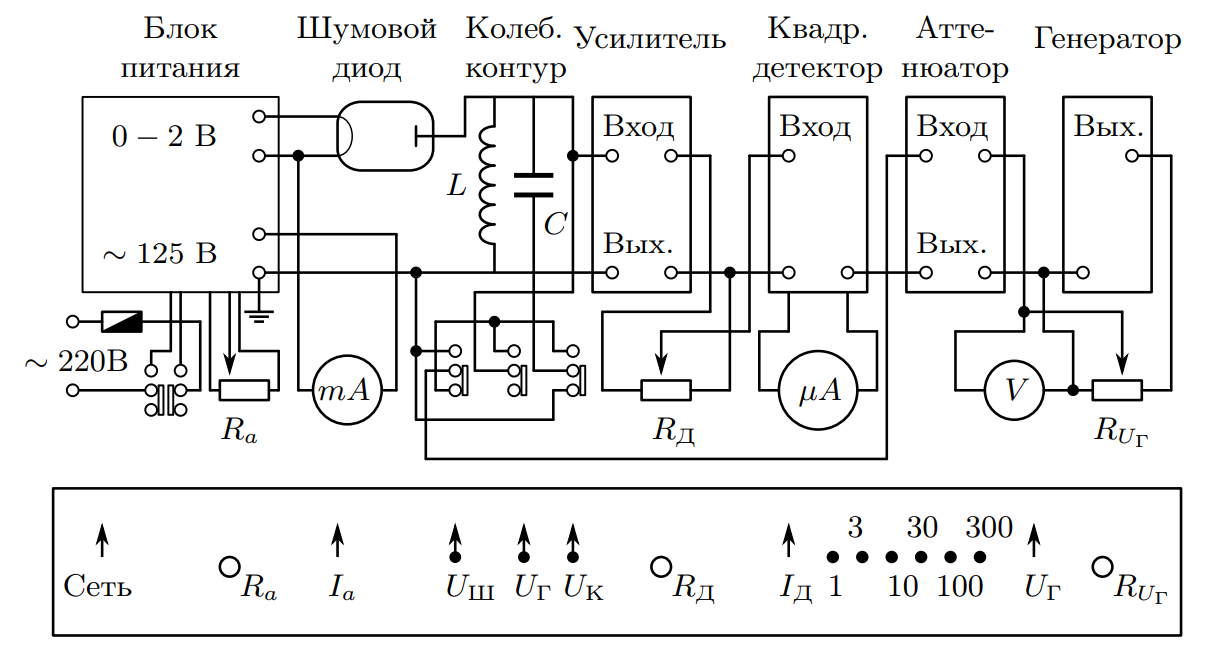
\includegraphics [scale=0.7]{ustanovka.png}}
		\caption{Схема установки для измерения дробового шума.}
	\end{figure}
	
	\newpage
	\textbf{Результаты измерений и обработка данных: }\\
	
	\textit{Проверка квадратичности детектора: }
	\begin{enumerate}
		
	\item Включим стенд в режим измерения напряжения генератора. Установим максимальную чувствительность квадратичного детектора и выберем предел измерений для вольтметра (100 мкВ аттенюатора). Изменяя выходное напряжение генератора, измерим зависимость тока квадратичного детектора $I_{\text{д}}$ от входного напряжения усилителя $U_{\text{г}}$. Полученные данные занесем в таблицу 1.
	
	\begin{longtable} {|c|c|c|c|c|c|c|c|c|c|}
		\hline
		$U_{\text{г}}$, мкВ & 60 & 62 & 64 & 66 & 68 & 70 & 72 & 74 & 76     \\ \hline
		$I_{\text{д}}$, мкА& 38 & 42 & 44 & 47 & 50 & 53 & 56 & 60 & 63\\ \hline
		\hline
		$U_{\text{г}}$, мкВ & 78 & 80 & 82 & 84 & 86 & 88 & 90 & 92 & 94\\ \hline
		$I_{\text{д}}$, мкА& 66 & 70 & 74 & 79 & 83 & 87 & 91 & 96 & 100\\ \hline
		\caption{Зависимость $I_{\text{д}}(U_{\text{г}})$, $\sigma_{U_{\text{г}}} = 1$ мкВ, $\sigma_{I_{\text{д}}} = 1$ мкА}
	\end{longtable}
	
	\item По полученным данным построим  график зависимости $I_{\text{д}}(U_{\text{г}})$
	\begin{figure}[H]
		\center{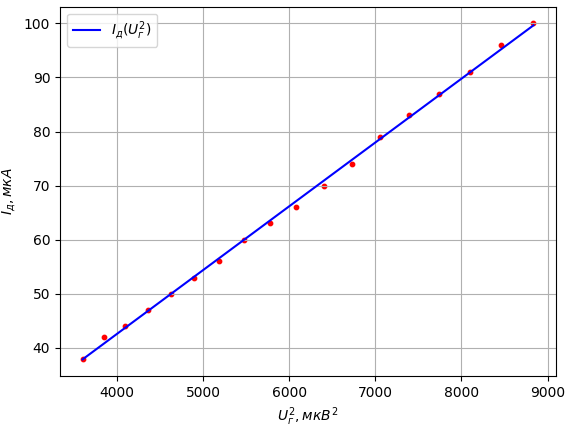
\includegraphics [scale=1]{Id(Ug).png}}
		\caption{График зависимости тока квадратичного детектора от квадрата входного напряжения усилителя}
	\end{figure}
	\newpage
	\textit{Измерение напряжения шума: }
	 
	\item Для различных значений анодного тока $I_a$ определим эффективное напряжение. Для этого установим произвольное значение шумового тока $I_{\text{д}}$. Для пересчёта отклика детектора на шум в единицы напряжения подключим к усилителю генератор напряжений вместо шумового диода. Установим то же значение тока $I_{\text{д}}$, которое было выбрано в режиме измерения шума, тогда значение на вольтметре будет искомым напряжением. Полученные значения занесем в таблицы 2 и 3.
	
	\begin{table}[H]
	\begin{center}
	\begin{tabular} {|c|c|c|}
		\hline
		& $I_{\text{д}}$, мкА & $U^{\text{эфф}}_1$, мкВ \\ \hline
		\multirow{5}{*}{$I_a = 1$, мА} & 75 & 80 \\ \cline{2-3}
		& 70 & 76 \\ \cline{2-3}
		& 60 & 75 \\ \cline{2-3}
		& 50 & 74 \\ \cline{2-3}
		& 40 & 74 \\ \hline
	\end{tabular}
	\begin{tabular} {|c|c|c|}
		\hline
		& $I_{\text{д}}$, мкА & $U^{\text{эфф}}_2$, мкВ \\ \hline
		\multirow{5}{*}{$I_a = 2$, мА} & 40 & 100 \\ \cline{2-3}
		& 50 & 105 \\ \cline{2-3}
		& 60 & 105 \\ \cline{2-3}
		& 70 & 105 \\ \cline{2-3}
		& 80 & 105 \\ \hline
	\end{tabular}

	\begin{tabular} {|c|c|c|}
		\hline
		& $I_{\text{д}}$, мкА & $U^{\text{эфф}}_2$, мкВ \\ \hline
		\multirow{5}{*}{$I_a = 3$, мА} & 40 & 120 \\ \cline{2-3}
		& 50 & 120 \\ \cline{2-3}
		& 60 & 120 \\ \cline{2-3}
		& 70 & 120 \\ \cline{2-3}
		& 80 & 125 \\ \hline
	\end{tabular}
	\begin{tabular} {|c|c|c|}
		\hline
		& $I_{\text{д}}$, мкА & $U^{\text{эфф}}_2$, мкВ \\ \hline
		\multirow{5}{*}{$I_a = 4$, мА} & 40 & 130 \\ \cline{2-3}
		& 50 & 130 \\ \cline{2-3}
		& 60 & 135 \\ \cline{2-3}
		& 70 & 135 \\ \cline{2-3}
		& 80 & 140 \\ \hline
	\end{tabular}
	\end{center}
	\caption{Значения для эффективного напряжения в зависимости от шумового тока. $\sigma_{I_{\text{а}}} = 0,1$ мА , $\sigma_{I_{\text{д}}} = 1$ мкА, $\sigma_{U^{\text{эфф}}_1} = 1$ мкВ, $\sigma_{U^{\text{эфф}}_2} = 5$ мкВ}
	\end{table}

	\textit{Измерение добротности контура: }
	
	\item Для тех же анодных токов из предыдущего пункта установим режим измерения напряжения на контуре при его последовательном возбуждении. При нулевом напряжении на вольтметре подберем чувствительность детектора: установим стрелку микроамперметра детектора на любое целое деление.Измерим приращение тока детектора $\Delta I_{\text{д}}$ при изменении напряжения генератора от нуля до любого напряжения $V_1$. Затем включим режим измерения напряжения на генераторе и подберем напряжение $V_2$, при котором
	ток квадратичного детектора равен приращению $\Delta I_{\text{д}}$ в режиме измерения сигнала с контура. Тогда добротность контура равна $ Q =  \frac{U_k}{U_{\text{г}}}$. Таким образом мы сможем посчитать заряд электрона по формуле(8). Полученные результаты занесем в таблицы 3 и 4.
	
	\begin{longtable} {|c|c|c|c|c|c|}
		\hline
		$I_{\text{a}}$, мА& $I^{\text{д}}_0$, мкА & $I^{\text{д}}_1$, мкА & $ U^{\text{г}}_1 $, мкВ  &$ U^{\text{г}}_2 $, мкВ  & $Q$\\ \hline
		
		\multirow{4}{*}{1} & 70 & 89 & 0,20 & 46 & 230 \\ \cline{2-6}
		  & 50 & 70 & 0,30 & 56 & 187 \\ \cline{2-6}
		  & 40 & 50 & 0,20 & 41 & 205 \\ \cline{2-6}
		  & 60 & 90 & 0,34 & 62 & 182 \\ \hline
		  \hline
		\multirow{4}{*}{2} & 40 & 60 & 0,50 & 75 & 150 \\ \cline{2-6}
		& 50 & 70 & 0,40 & 68 & 170 \\ \cline{2-6}
		& 60 & 80 & 0,36 & 64 & 178 \\ \cline{2-6}
		& 70 & 90 & 0,37 & 59 & 160 \\ \hline
		
		\hline
		$I_{\text{a}}$, мА& $I^{\text{д}}_0$, мкА & $I^{\text{д}}_1$, мкА & $ U^{\text{г}}_1 $, мкВ  &$ U^{\text{г}}_2 $, мкВ  & $Q$\\ \hline
		
		\multirow{4}{*}{3} & 40 & 60 & 0,70 & 86 & 123 \\ \cline{2-6}
		& 50 & 70 & 0,57 & 76 & 133 \\ \cline{2-6}
		& 60 & 80 & 0,52 & 72 & 138 \\ \cline{2-6}
		& 70 & 90 & 0,44 & 65 & 148 \\ \hline
		\hline
		\multirow{4}{*}{4} & 40 & 60 & 0,88 & 96 & 109 \\ \cline{2-6}
		& 50 & 70 & 0,84 & 87 & 104 \\ \cline{2-6}
		& 60 & 80 & 0,68 & 76 & 112 \\ \cline{2-6}
		& 70 & 90 & 0,63 & 72 & 114 \\ \hline
		
		\caption{Значения добротности контура, $\sigma_{I_{\text{а}}} = 0,1$ мА, $\sigma_{I_{\text{д}}} = 1$ мкА, $\sigma_{U^{\text{г}}_1} = 0,01$ мкВ, $\sigma_{U^{\text{г}}_2} = 1$ мкВ, $\varepsilon_Q = 4\%$}
	\end{longtable}
	
	
	\begin{longtable} {|c|c|c|c|c|}
		\hline
		$I_{\text{a}}$, мА& $\langle U_{\text{эфф}} \rangle$, мкВ & $\langle Q \rangle$ & $e$, $10^{-19}$ Кл & $\langle e \rangle$, $10^{-19}$ Кл \\ \hline
		
		1 & 76 & 201 & 0,65 & \multirow{4}{*}{0,78 $\pm$ 0,09} \\ \cline{1-4}
		2 & 104 & 165 & 0,74 &  \\ \cline{1-4}
		3 & 121 & 136 & 0,81 &  \\ \cline{1-4}
		4 & 134 & 110 & 0,92 &  \\ \hline
		\caption{}
	\end{longtable}
	
	
	
	
	
	
	
	
	
	
	
	
	
	
	
	
	
	\end{enumerate}
	
	
	
	\end{document}
